\documentclass[en]{article}
\usepackage[left=2.2cm,right=2.2cm,top=2.5cm,bottom=2.5cm]{geometry}
\usepackage[utf8]{inputenc}
%\usepackage{minted}
\usepackage{booktabs}
\usepackage{commath}
\usepackage{float}
\usepackage{mathtools}
\usepackage{amsthm}


\usepackage[binary-units=true]{siunitx}

%\newcommand{\py}[1]{\mintinline{python}{#1}}

\title{Artificial Intelligence (\texttt{LINGI2261}) \\ Assignment 2 --- Group 13}
\author{Martin Braquet, Gilles Peiffer}

\begin{document}

\maketitle

\section{Alpha-Beta search}

\subsection{MiniMax algorithm}

\begin{figure}[H]
 \centering
 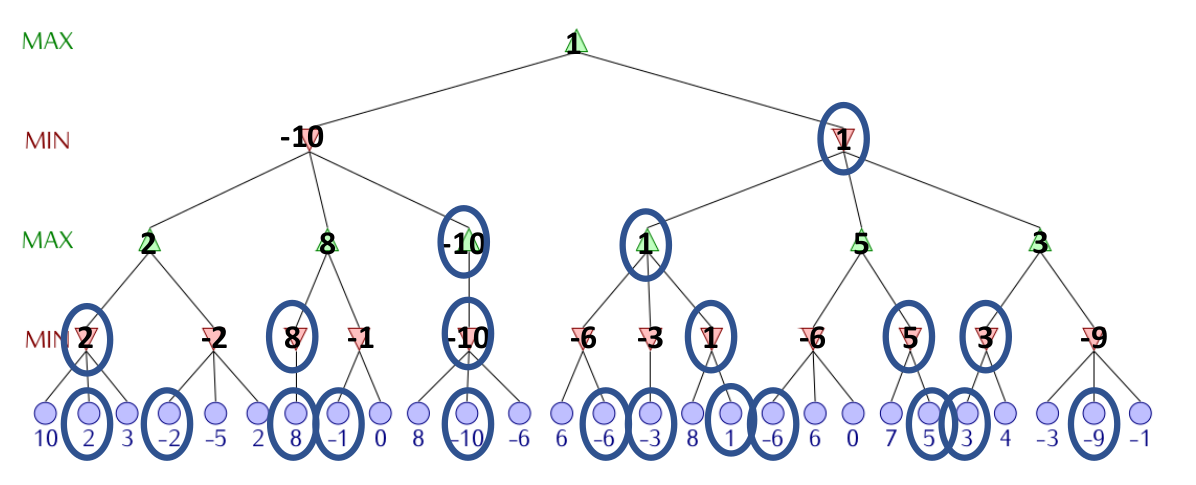
\includegraphics[width=\textwidth]{MiniMax.png}
 \caption{Minimax algorithm}
 \label{fig:minimax}
\end{figure}


\subsection{Alpha-Beta algorithm (left to right)}

\begin{figure}[H]
 \centering
 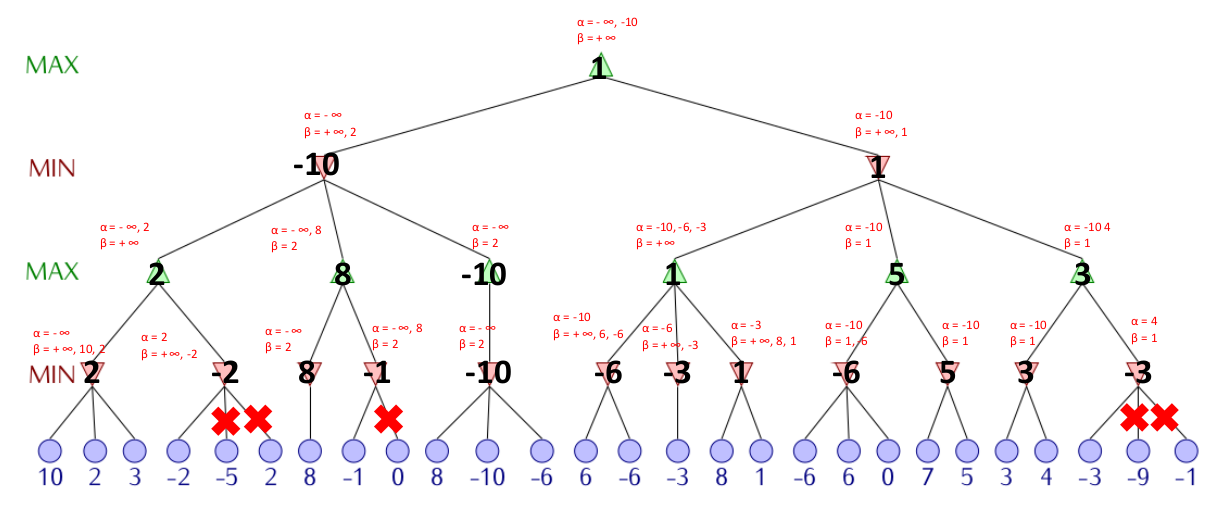
\includegraphics[width=\textwidth]{Alphabeta.png}
 \caption{Alpha-Beta algorithm (left to right)}
 \label{fig:alphabeta}
\end{figure}


\subsection{Alpha-Beta algorithm (right to left)}

\begin{figure}[H]
 \centering
 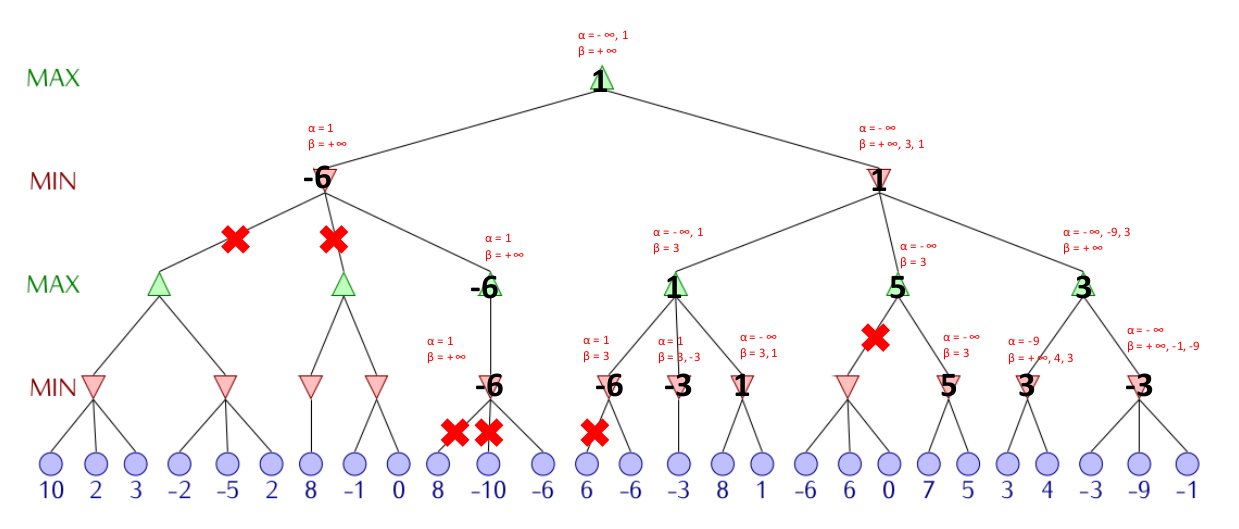
\includegraphics[width=\textwidth]{Alphabeta_reverse.png}
 \caption{Alpha-Beta algorithm (right to left)}
 \label{fig:alphabeta_reverse}
\end{figure}


\subsection{Alpha-Beta algorithm (ordered)}

\begin{figure}[H]
 \centering
 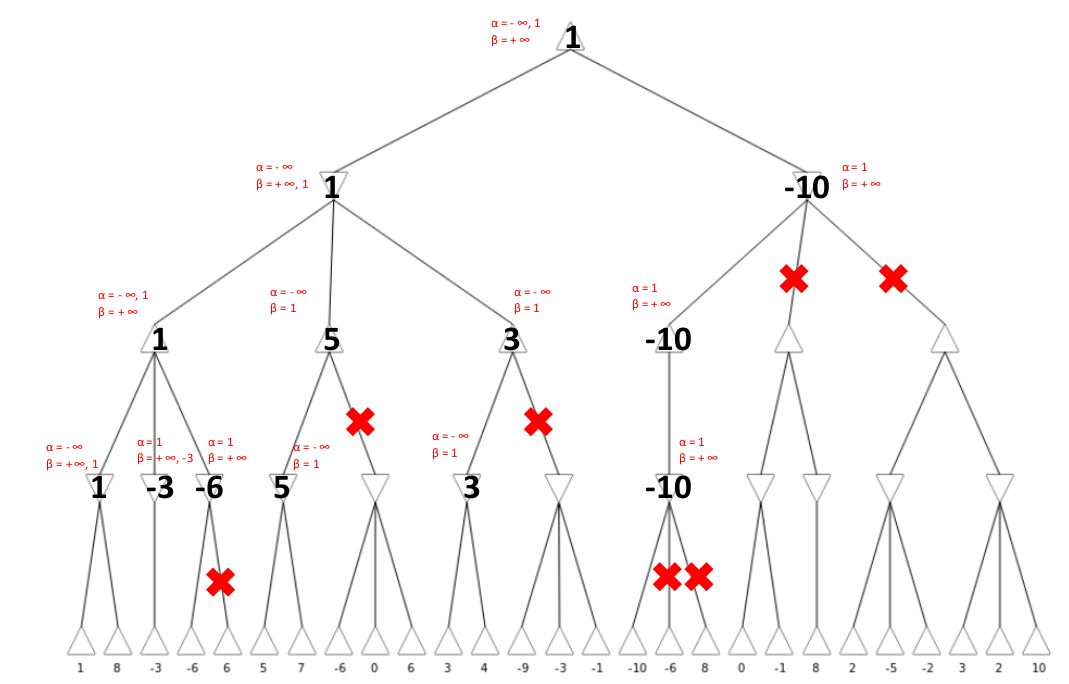
\includegraphics[width=\textwidth]{Alphabeta_ordered.png}
 \caption{Alpha-Beta algorithm}
 \label{fig:alphabeta_ordered}
\end{figure}

\subsection{Alpha-Beta for more than two players}

\end{document}
